% future/cpu.tex
% mainfile: ../perfbook.tex
% SPDX-License-Identifier: CC-BY-SA-3.0

\section{The Future of CPU Technology Ain't What it Used to Be}
\label{sec:future:The Future of CPU Technology Ain't What it Used to Be}
%
\epigraph{A great future behind him.}{\emph{David Maraniss}}

과거의 것들은 수많은 해의 경험을 거친 렌즈로 보면 무척 간단하고 순수해
보입니다.
그리고 2000년대 초는 \IX{Moore's Law} 가 그때는 전통적이던 CPU 클락 주파수의
증가를 가져다 주는 것에 대한 임박한 실패로부터 결백했습니다.
오, 기술의 한계에 대한 가끔의 경고가 있긴 했습니다만 그런 경고는 수십년째
들려오고 있었습니다.
그걸 고려하고 다음 시나리오들을 생각해 봅시다:

\iffalse

Years past always seem so simple and innocent when viewed through the
lens of many years of experience.
And the early 2000s were for the most part innocent of the impending
failure of \IX{Moore's Law} to continue delivering the then-traditional
increases in CPU clock frequency.
Oh, there were the occasional warnings about the limits of technology,
but such warnings had been sounded for decades.
With that in mind, consider the following scenarios:

\fi

\begin{figure}[tb]
\centering
\resizebox{3in}{!}{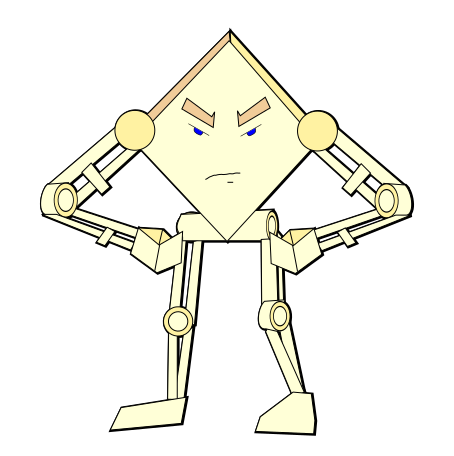
\includegraphics{cartoons/r-2014-CPU-future-uniprocessor-uber-alles}}
\caption{Uniprocessor \"Uber Alles}
\ContributedBy{Figure}{fig:future:Uniprocessor \"Uber Alles}{Melissa Broussard}
\end{figure}

\begin{figure}[tb]
\centering
\resizebox{2.6in}{!}{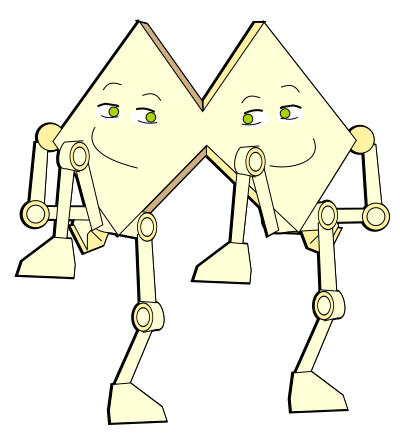
\includegraphics{cartoons/r-2014-CPU-Future-Multithreaded-Mania}}
\caption{Multithreaded Mania}
\ContributedBy{Figure}{fig:future:Multithreaded Mania}{Melissa Broussard}
\end{figure}

\begin{figure}[tb]
\centering
\resizebox{2.5in}{!}{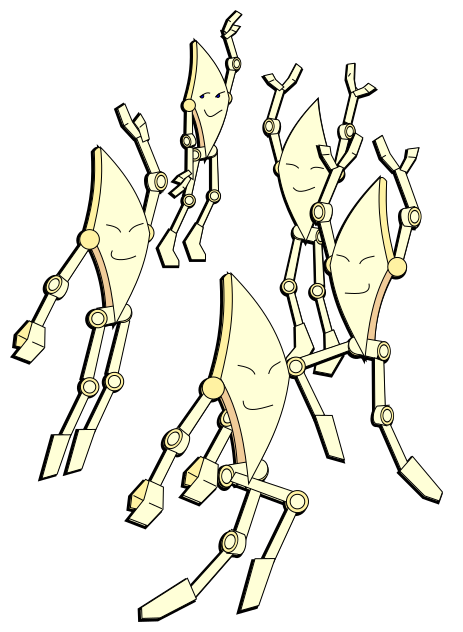
\includegraphics{cartoons/r-2014-CPU-Future-More-of-the-Same}}
\caption{More of the Same}
\ContributedBy{Figure}{fig:future:More of the Same}{Melissa Broussard}
\end{figure}

\begin{figure}[tb]
\centering
\resizebox{3in}{!}{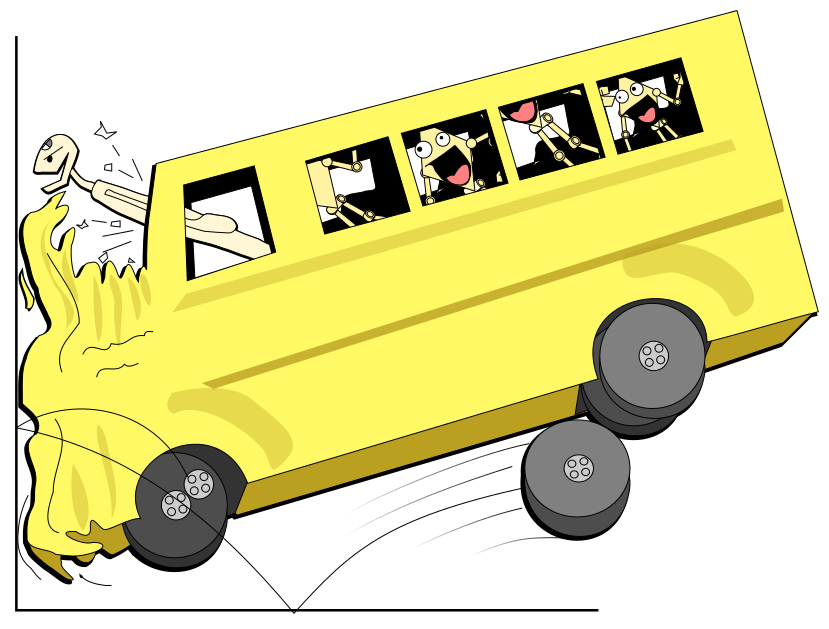
\includegraphics{cartoons/r-2014-CPU-Future-Crash-dummies}}
\caption{Crash Dummies Slamming into the Memory Wall}
\ContributedBy{Figure}{fig:future:Crash Dummies Slamming into the Memory Wall}{Melissa Broussard}
\end{figure}

\begin{figure}[tb]
\centering
\resizebox{3in}{!}{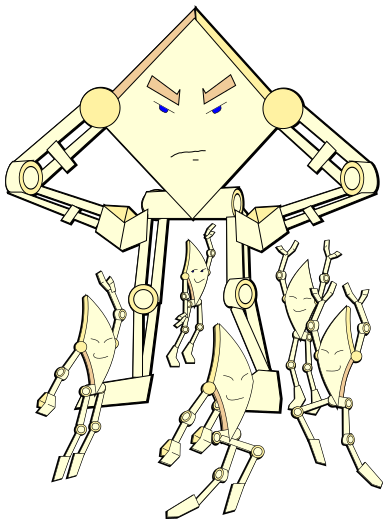
\includegraphics{cartoons/r-2021-CPU-future-astounding-accelerator}}
\caption{Astounding Accelerators}
\ContributedBy{Figure}{fig:future:Astounding Accelerators}{Melissa Broussard, remixed}
\end{figure}

\begin{enumerate}
\item	Uniprocessor \"Uber Alles
	(\Cref{fig:future:Uniprocessor \"Uber Alles}),
\item	Multithreaded Mania
	(\Cref{fig:future:Multithreaded Mania}),
\item	More of the Same
	(\Cref{fig:future:More of the Same}), and
\item	Crash Dummies Slamming into the Memory Wall
	(\Cref{fig:future:Crash Dummies Slamming into the Memory Wall}).
\item	Astounding Accelerators
	(\Cref{fig:future:Astounding Accelerators}).
\end{enumerate}

이 시나리오 각각은 다음 섹션들에서 다루어집니다.

\iffalse

Each of these scenarios is covered in the following sections.

\fi

\subsection{Uniprocessor \"Uber Alles}
\label{sec:future:Uniprocessor \"Uber Alles}

As was said in 2004~\cite{PaulEdwardMcKenneyPhD}:

\begin{quote}
	In this scenario, the combination of \IXalt{Moore's-Law}{Moore's Law}
	increases in CPU
	clock rate and continued progress in horizontally scaled computing
	render SMP systems irrelevant.
	This scenario is therefore dubbed ``Uniprocessor \"Uber
	Alles'', literally, uniprocessors above all else.

	These uniprocessor systems would be subject only to instruction
	overhead, since memory barriers, cache thrashing, and contention
	do not affect single-CPU systems.
	In this scenario, RCU is useful only for niche applications, such
	as interacting with NMIs.
	It is not clear that an operating system lacking RCU would see
	the need to adopt it, although operating
	systems that already implement RCU might continue to do so.

	However, recent progress with multithreaded CPUs seems to indicate
	that this scenario is quite unlikely.
\end{quote}

Unlikely indeed!
But the larger software community was reluctant to accept the fact that
they would need to embrace parallelism, and so it was some time before
this community concluded that the ``free lunch'' of
\IXalt{Moore's-Law}{Moore's Law}-induced
CPU core-clock frequency increases was well and truly finished.
Never forget: belief is an emotion, not necessarily the result of a
rational technical thought process!

\subsection{Multithreaded Mania}
\label{sec:future:Multithreaded Mania}

Also from 2004~\cite{PaulEdwardMcKenneyPhD}:

\begin{quote}
	A less-extreme variant of Uniprocessor \"Uber Alles features
	uniprocessors with hardware multithreading, and in fact
	multithreaded CPUs are now standard for many desktop and laptop
	computer systems.
	The most aggressively multithreaded CPUs share all levels of
	cache hierarchy, thereby eliminating CPU-to-CPU memory latency,
	in turn greatly reducing the performance penalty for traditional
	synchronization mechanisms.
	However, a multithreaded CPU would still incur overhead due to
	contention and to pipeline stalls caused by memory barriers.
	Furthermore, because all hardware threads share all levels
	of cache, the cache available to a given hardware thread is a
	fraction of what it would be on an equivalent single-threaded
	CPU, which can degrade performance for applications with large
	cache footprints.
	There is also some possibility that the restricted amount of cache
	available will cause RCU-based algorithms to incur performance
	penalties due to their grace-period-induced additional memory
	consumption.
	Investigating this possibility is future work.

	However, in order to avoid such performance degradation, a number
	of multithreaded CPUs and multi-CPU chips partition at least
	some of the levels of cache on a per-hardware-thread basis.
	This increases the amount of cache available to each hardware
	thread, but re-introduces memory latency for cachelines that
	are passed from one hardware thread to another.
\end{quote}

And we all know how this story has played out, with multiple multi-threaded
cores on a single die plugged into a single socket, with varying degrees
of optimization for lower numbers of active threads per core.
The question then becomes whether or not future shared-memory systems will
always fit into a single socket.

\subsection{More of the Same}
\label{sec:meas:More of the Same}

Again from 2004~\cite{PaulEdwardMcKenneyPhD}:

\begin{quote}
	The More-of-the-Same scenario assumes that the memory-latency
	ratios will remain roughly where they are today.

	This scenario actually represents a change, since to have more
	of the same, interconnect performance must begin keeping up
	with the \IXalt{Moore's-Law}{Moore's Law} increases in core CPU performance.
	In this scenario, overhead due to pipeline stalls, memory latency,
	and contention remains significant, and RCU retains the high
	level of applicability that it enjoys today.
\end{quote}

And the change has been the ever-increasing levels of integration
that \IX{Moore's Law} is still providing.
But longer term, which will it be?
More CPUs per die?
Or more I/O, cache, and memory?

Servers seem to be choosing the former, while embedded systems on a chip
(SoCs) continue choosing the latter.

\subsection{Crash Dummies Slamming into the Memory Wall}
\label{sec:future:Crash Dummies Slamming into the Memory Wall}

\begin{figure}[tbp]
\centering
\epsfxsize=3in
\epsfbox{future/latencytrend}
% from Ph.D. thesis: related/latencytrend.eps
\caption{Instructions per Local Memory Reference for Sequent Computers}
\label{fig:future:Instructions per Local Memory Reference for Sequent Computers}
\end{figure}

\begin{figure}[htbp]
\centering
\epsfxsize=3in
\epsfbox{future/be-lb-n4-rf-all}
% from Ph.D. thesis: an/plots/be-lb-n4-rf-all.eps
\caption{Breakevens vs. $r$, $\lambda$ Large, Four CPUs}
\label{fig:future:Breakevens vs. r; lambda Large; Four CPUs}
\end{figure}

\begin{figure}[htbp]
\centering
\epsfxsize=3in
\epsfbox{future/be-lw-n4-rf-all}
% from Ph.D. thesis: an/plots/be-lw-n4-rf-all.eps
\caption{Breakevens vs. $r$, $\lambda$ Small, Four CPUs}
\label{fig:future:Breakevens vs. r; Worst-Case lambda; Four CPUs}
\end{figure}

And one more quote from 2004~\cite{PaulEdwardMcKenneyPhD}:

\begin{quote}
	If the memory-latency trends shown in
	\cref{fig:future:Instructions per Local Memory Reference for Sequent Computers}
	continue, then memory latency will continue to grow relative
	to instruction-execution overhead.
	Systems such as Linux that have significant use of RCU will find
	additional use of RCU to be profitable, as shown in
	\cref{fig:future:Breakevens vs. r; lambda Large; Four CPUs}.
	As can be seen in this figure, if RCU is heavily used, increasing
	memory-latency ratios give RCU an increasing advantage over other
	synchronization mechanisms.
	In contrast, systems with minor
	use of RCU will require increasingly high degrees of read intensity
	for use of RCU to pay off, as shown in
	\cref{fig:future:Breakevens vs. r; Worst-Case lambda; Four CPUs}.
	As can be seen in this figure, if RCU is lightly used,
	increasing memory-latency ratios
	put RCU at an increasing disadvantage compared to other synchronization
	mechanisms.
	Since Linux has been observed with over 1,600 callbacks per grace
	period under heavy load~\cite{Sarma04c},
	it seems safe to say that Linux falls into the former category.
\end{quote}

On the one hand, this passage failed to anticipate the cache-warmth
issues that RCU can suffer from in workloads with significant update
intensity, in part because it seemed unlikely that RCU would really
be used for such workloads.
In the event, the \co{SLAB_TYPESAFE_BY_RCU} has been pressed into
service in a number of instances where these cache-warmth issues would
otherwise be problematic, as has sequence locking.
On the other hand, this passage also failed to anticipate that
RCU would be used to reduce scheduling latency or for security.

Much of the data generated for this book was collected on an eight-socket
system with 28 cores per socket and two hardware threads per core, for
a total of 448 hardware threads.
The idle-system memory latencies are less than one microsecond, which
are no worse than those of similar-sized systems of the year 2004.
Some claim that these latencies approach a microsecond only because of
the x86 CPU family's relatively strong memory ordering, but it may be
some time before that particular argument is settled.

\subsection{Astounding Accelerators}
\label{sec:future:Astounding Accelerators}

The potential of hardware accelerators was not quite as clear in 2004
as it is in 2021, so this section has no quote.
However, the November 2020 Top 500 list~\cite{Top500} features a great
many accelerators, so one could argue that this section is a view of
the present rather than of the future.
The same could be said of most of the preceding sections.

Hardware accelerators are being put to many other uses, including
encryption, compression, machine learning.

In short, beware of prognostications, including those in the remainder
of this chapter.
